\documentclass[1p]{elsarticle_modified}
%\bibliographystyle{elsarticle-num}

%\usepackage[colorlinks]{hyperref}
%\usepackage{abbrmath_seonhwa} %\Abb, \Ascr, \Acal ,\Abf, \Afrak
\usepackage{amsfonts}
\usepackage{amssymb}
\usepackage{amsmath}
\usepackage{amsthm}
\usepackage{scalefnt}
\usepackage{amsbsy}
\usepackage{kotex}
\usepackage{caption}
\usepackage{subfig}
\usepackage{color}
\usepackage{graphicx}
\usepackage{xcolor} %% white, black, red, green, blue, cyan, magenta, yellow
\usepackage{float}
\usepackage{setspace}
\usepackage{hyperref}

\usepackage{tikz}
\usetikzlibrary{arrows}

\usepackage{multirow}
\usepackage{array} % fixed length table
\usepackage{hhline}

%%%%%%%%%%%%%%%%%%%%%
\makeatletter
\renewcommand*\env@matrix[1][\arraystretch]{%
	\edef\arraystretch{#1}%
	\hskip -\arraycolsep
	\let\@ifnextchar\new@ifnextchar
	\array{*\c@MaxMatrixCols c}}
\makeatother %https://tex.stackexchange.com/questions/14071/how-can-i-increase-the-line-spacing-in-a-matrix
%%%%%%%%%%%%%%%

\usepackage[normalem]{ulem}

\newcommand{\msout}[1]{\ifmmode\text{\sout{\ensuremath{#1}}}\else\sout{#1}\fi}
%SOURCE: \msout is \stkout macro in https://tex.stackexchange.com/questions/20609/strikeout-in-math-mode

\newcommand{\cancel}[1]{
	\ifmmode
	{\color{red}\msout{#1}}
	\else
	{\color{red}\sout{#1}}
	\fi
}

\newcommand{\add}[1]{
	{\color{blue}\uwave{#1}}
}

\newcommand{\replace}[2]{
	\ifmmode
	{\color{red}\msout{#1}}{\color{blue}\uwave{#2}}
	\else
	{\color{red}\sout{#1}}{\color{blue}\uwave{#2}}
	\fi
}

\newcommand{\Sol}{\mathcal{S}} %segment
\newcommand{\D}{D} %diagram
\newcommand{\A}{\mathcal{A}} %arc


%%%%%%%%%%%%%%%%%%%%%%%%%%%%%5 test

\def\sl{\operatorname{\textup{SL}}(2,\Cbb)}
\def\psl{\operatorname{\textup{PSL}}(2,\Cbb)}
\def\quan{\mkern 1mu \triangleright \mkern 1mu}

\theoremstyle{definition}
\newtheorem{thm}{Theorem}[section]
\newtheorem{prop}[thm]{Proposition}
\newtheorem{lem}[thm]{Lemma}
\newtheorem{ques}[thm]{Question}
\newtheorem{cor}[thm]{Corollary}
\newtheorem{defn}[thm]{Definition}
\newtheorem{exam}[thm]{Example}
\newtheorem{rmk}[thm]{Remark}
\newtheorem{alg}[thm]{Algorithm}

\newcommand{\I}{\sqrt{-1}}
\begin{document}

%\begin{frontmatter}
%
%\title{Boundary parabolic representations of knots up to 8 crossings}
%
%%% Group authors per affiliation:
%\author{Yunhi Cho} 
%\address{Department of Mathematics, University of Seoul, Seoul, Korea}
%\ead{yhcho@uos.ac.kr}
%
%
%\author{Seonhwa Kim} %\fnref{s_kim}}
%\address{Center for Geometry and Physics, Institute for Basic Science, Pohang, 37673, Korea}
%\ead{ryeona17@ibs.re.kr}
%
%\author{Hyuk Kim}
%\address{Department of Mathematical Sciences, Seoul National University, Seoul 08826, Korea}
%\ead{hyukkim@snu.ac.kr}
%
%\author{Seokbeom Yoon}
%\address{Department of Mathematical Sciences, Seoul National University, Seoul, 08826,  Korea}
%\ead{sbyoon15@snu.ac.kr}
%
%\begin{abstract}
%We find all boundary parabolic representation of knots up to 8 crossings.
%
%\end{abstract}
%\begin{keyword}
%    \MSC[2010] 57M25 
%\end{keyword}
%
%\end{frontmatter}

%\linenumbers
%\tableofcontents
%
\newcommand\colored[1]{\textcolor{white}{\rule[-0.35ex]{0.8em}{1.4ex}}\kern-0.8em\color{red} #1}%
%\newcommand\colored[1]{\textcolor{white}{ #1}\kern-2.17ex	\textcolor{white}{ #1}\kern-1.81ex	\textcolor{white}{ #1}\kern-2.15ex\color{red}#1	}

{\Large $\underline{12a_{1016}~(K12a_{1016})}$}

\setlength{\tabcolsep}{10pt}
\renewcommand{\arraystretch}{1.6}
\vspace{1cm}\begin{tabular}{m{100pt}>{\centering\arraybackslash}m{274pt}}
\multirow{5}{120pt}{
	\centering
	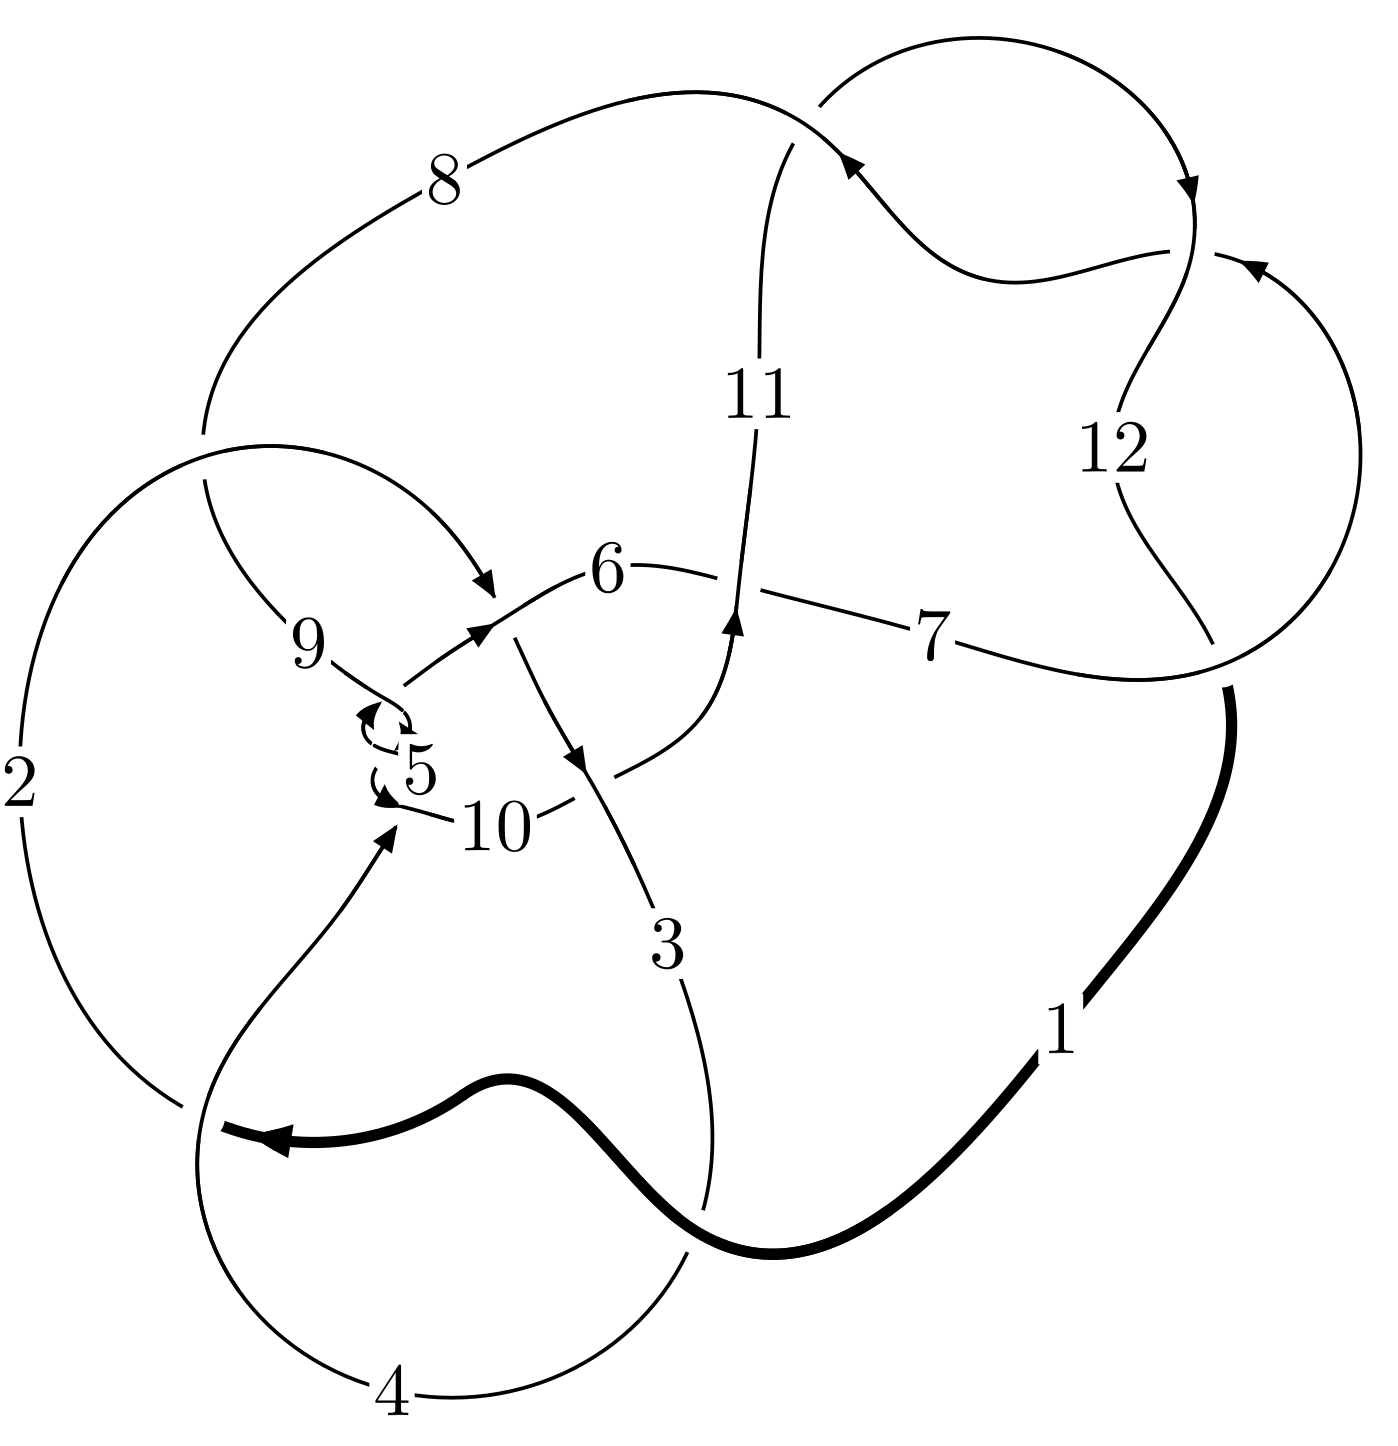
\includegraphics[width=112pt]{../../../GIT/diagram.site/Diagrams/png/1817_12a_1016.png}\\
\ \ \ A knot diagram\footnotemark}&
\allowdisplaybreaks
\textbf{Linearized knot diagam} \\
\cline{2-2}
 &
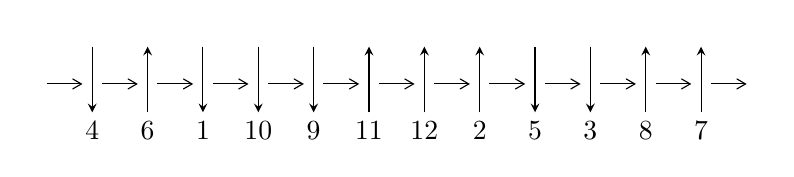
\begin{tikzpicture}[x=20pt, y=17pt]
	% nodes
	\node (C0) at (0, 0) {};
	\node (C1) at (1, 0) {};
	\node (C1U) at (1, +1) {};
	\node (C1D) at (1, -1) {4};

	\node (C2) at (2, 0) {};
	\node (C2U) at (2, +1) {};
	\node (C2D) at (2, -1) {6};

	\node (C3) at (3, 0) {};
	\node (C3U) at (3, +1) {};
	\node (C3D) at (3, -1) {1};

	\node (C4) at (4, 0) {};
	\node (C4U) at (4, +1) {};
	\node (C4D) at (4, -1) {10};

	\node (C5) at (5, 0) {};
	\node (C5U) at (5, +1) {};
	\node (C5D) at (5, -1) {9};

	\node (C6) at (6, 0) {};
	\node (C6U) at (6, +1) {};
	\node (C6D) at (6, -1) {11};

	\node (C7) at (7, 0) {};
	\node (C7U) at (7, +1) {};
	\node (C7D) at (7, -1) {12};

	\node (C8) at (8, 0) {};
	\node (C8U) at (8, +1) {};
	\node (C8D) at (8, -1) {2};

	\node (C9) at (9, 0) {};
	\node (C9U) at (9, +1) {};
	\node (C9D) at (9, -1) {5};

	\node (C10) at (10, 0) {};
	\node (C10U) at (10, +1) {};
	\node (C10D) at (10, -1) {3};

	\node (C11) at (11, 0) {};
	\node (C11U) at (11, +1) {};
	\node (C11D) at (11, -1) {8};

	\node (C12) at (12, 0) {};
	\node (C12U) at (12, +1) {};
	\node (C12D) at (12, -1) {7};
	\node (C13) at (13, 0) {};

	% arrows
	\draw[->,>={angle 60}]
	(C0) edge (C1) (C1) edge (C2) (C2) edge (C3) (C3) edge (C4) (C4) edge (C5) (C5) edge (C6) (C6) edge (C7) (C7) edge (C8) (C8) edge (C9) (C9) edge (C10) (C10) edge (C11) (C11) edge (C12) (C12) edge (C13) ;	\draw[->,>=stealth]
	(C1U) edge (C1D) (C2D) edge (C2U) (C3U) edge (C3D) (C4U) edge (C4D) (C5U) edge (C5D) (C6D) edge (C6U) (C7D) edge (C7U) (C8D) edge (C8U) (C9U) edge (C9D) (C10U) edge (C10D) (C11D) edge (C11U) (C12D) edge (C12U) ;
	\end{tikzpicture} \\
\hhline{~~} \\& 
\textbf{Solving Sequence} \\ \cline{2-2} 
 &
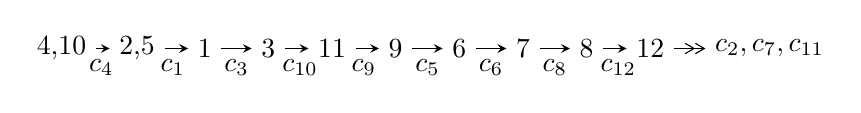
\begin{tikzpicture}[x=23pt, y=7pt]
	% node
	\node (A0) at (-1/8, 0) {4,10};
	\node (A1) at (17/16, 0) {2,5};
	\node (A2) at (17/8, 0) {1};
	\node (A3) at (25/8, 0) {3};
	\node (A4) at (33/8, 0) {11};
	\node (A5) at (41/8, 0) {9};
	\node (A6) at (49/8, 0) {6};
	\node (A7) at (57/8, 0) {7};
	\node (A8) at (65/8, 0) {8};
	\node (A9) at (73/8, 0) {12};
	\node (C1) at (1/2, -1) {$c_{4}$};
	\node (C2) at (13/8, -1) {$c_{1}$};
	\node (C3) at (21/8, -1) {$c_{3}$};
	\node (C4) at (29/8, -1) {$c_{10}$};
	\node (C5) at (37/8, -1) {$c_{9}$};
	\node (C6) at (45/8, -1) {$c_{5}$};
	\node (C7) at (53/8, -1) {$c_{6}$};
	\node (C8) at (61/8, -1) {$c_{8}$};
	\node (C9) at (69/8, -1) {$c_{12}$};
	\node (A10) at (11, 0) {$c_{2},c_{7},c_{11}$};

	% edge
	\draw[->,>=stealth]	
	(A0) edge (A1) (A1) edge (A2) (A2) edge (A3) (A3) edge (A4) (A4) edge (A5) (A5) edge (A6) (A6) edge (A7) (A7) edge (A8) (A8) edge (A9) ;
	\draw[->>,>={angle 60}]	
	(A9) edge (A10);
\end{tikzpicture} \\ 

\end{tabular} \\

\footnotetext{
The image of knot diagram is generated by the software ``\textbf{Draw programme}" developed by Andrew Bartholomew(\url{http://www.layer8.co.uk/maths/draw/index.htm\#Running-draw}), where we modified some parts for our purpose(\url{https://github.com/CATsTAILs/LinksPainter}).
}\phantom \\ \newline 
\centering \textbf{Ideals for irreducible components\footnotemark of $X_{\text{par}}$} 
 
\begin{align*}
I^u_{1}&=\langle 
-2.43965\times10^{142} u^{91}-2.96374\times10^{142} u^{90}+\cdots+1.68305\times10^{144} b+1.79998\times10^{144},\\
\phantom{I^u_{1}}&\phantom{= \langle  }3.24920\times10^{145} u^{91}+5.02902\times10^{145} u^{90}+\cdots+2.86119\times10^{145} a-3.31514\times10^{144},\;u^{92}+2 u^{91}+\cdots+2 u+1\rangle \\
I^u_{2}&=\langle 
b+1,\;- u^3-11 u^2+17 a-9 u-5,\;u^4+u^3+u^2+1\rangle \\
\\
\end{align*}
\raggedright * 2 irreducible components of $\dim_{\mathbb{C}}=0$, with total 96 representations.\\
\footnotetext{All coefficients of polynomials are rational numbers. But the coefficients are sometimes approximated in decimal forms when there is not enough margin.}
\newpage
\renewcommand{\arraystretch}{1}
\centering \section*{I. $I^u_{1}= \langle -2.44\times10^{142} u^{91}-2.96\times10^{142} u^{90}+\cdots+1.68\times10^{144} b+1.80\times10^{144},\;3.25\times10^{145} u^{91}+5.03\times10^{145} u^{90}+\cdots+2.86\times10^{145} a-3.32\times10^{144},\;u^{92}+2 u^{91}+\cdots+2 u+1 \rangle$}
\flushleft \textbf{(i) Arc colorings}\\
\begin{tabular}{m{7pt} m{180pt} m{7pt} m{180pt} }
\flushright $a_{4}=$&$\begin{pmatrix}1\\0\end{pmatrix}$ \\
\flushright $a_{10}=$&$\begin{pmatrix}0\\u\end{pmatrix}$ \\
\flushright $a_{2}=$&$\begin{pmatrix}-1.13561 u^{91}-1.75767 u^{90}+\cdots-7.01717 u+0.115866\\0.0144954 u^{91}+0.0176093 u^{90}+\cdots+0.109965 u-1.06947\end{pmatrix}$ \\
\flushright $a_{5}=$&$\begin{pmatrix}1\\u^2\end{pmatrix}$ \\
\flushright $a_{1}=$&$\begin{pmatrix}-1.12112 u^{91}-1.74006 u^{90}+\cdots-6.90720 u-0.953605\\0.0144954 u^{91}+0.0176093 u^{90}+\cdots+0.109965 u-1.06947\end{pmatrix}$ \\
\flushright $a_{3}=$&$\begin{pmatrix}-1.14289 u^{91}-1.76597 u^{90}+\cdots-7.02281 u+0.125248\\0.0106639 u^{91}+0.00260308 u^{90}+\cdots+0.0904560 u-1.08464\end{pmatrix}$ \\
\flushright $a_{11}=$&$\begin{pmatrix}-1.31145 u^{91}-3.32635 u^{90}+\cdots-11.3186 u-5.95210\\0.544767 u^{91}+1.07553 u^{90}+\cdots+3.57377 u+1.08287\end{pmatrix}$ \\
\flushright $a_{9}=$&$\begin{pmatrix}u\\u^3+u\end{pmatrix}$ \\
\flushright $a_{6}=$&$\begin{pmatrix}u^2+1\\u^4+2 u^2\end{pmatrix}$ \\
\flushright $a_{7}=$&$\begin{pmatrix}0.104548 u^{91}+0.533416 u^{90}+\cdots-1.42374 u+4.75175\\-0.210757 u^{91}-0.419015 u^{90}+\cdots-0.811424 u-0.740713\end{pmatrix}$ \\
\flushright $a_{8}=$&$\begin{pmatrix}-1.20284 u^{91}-2.85259 u^{90}+\cdots-5.65875 u-6.26189\\0.602208 u^{91}+1.20272 u^{90}+\cdots+4.08126 u+1.16263\end{pmatrix}$ \\
\flushright $a_{12}=$&$\begin{pmatrix}-0.519155 u^{91}-1.70050 u^{90}+\cdots-11.2427 u-3.96239\\0.285601 u^{91}+0.468224 u^{90}+\cdots+1.92592 u+0.636332\end{pmatrix}$\\&\end{tabular}
\flushleft \textbf{(ii) Obstruction class $= -1$}\\~\\
\flushleft \textbf{(iii) Cusp Shapes $= -4.11119 u^{91}-6.51477 u^{90}+\cdots-21.5680 u-8.41021$}\\~\\
\newpage\renewcommand{\arraystretch}{1}
\flushleft \textbf{(iv) u-Polynomials at the component}\newline \\
\begin{tabular}{m{50pt}|m{274pt}}
Crossings & \hspace{64pt}u-Polynomials at each crossing \\
\hline $$\begin{aligned}c_{1},c_{3}\end{aligned}$$&$\begin{aligned}
&u^{92}-5 u^{91}+\cdots-2416 u+289
\end{aligned}$\\
\hline $$\begin{aligned}c_{2}\end{aligned}$$&$\begin{aligned}
&u^{92}-7 u^{91}+\cdots-48824 u+4624
\end{aligned}$\\
\hline $$\begin{aligned}c_{4},c_{5},c_{9}\end{aligned}$$&$\begin{aligned}
&u^{92}+2 u^{91}+\cdots+2 u+1
\end{aligned}$\\
\hline $$\begin{aligned}c_{6}\end{aligned}$$&$\begin{aligned}
&u^{92}+2 u^{91}+\cdots-1508 u+740
\end{aligned}$\\
\hline $$\begin{aligned}c_{7},c_{11},c_{12}\end{aligned}$$&$\begin{aligned}
&u^{92}-2 u^{91}+\cdots-4 u+1
\end{aligned}$\\
\hline $$\begin{aligned}c_{8}\end{aligned}$$&$\begin{aligned}
&17(17 u^{92}-174 u^{91}+\cdots+130298 u+44509)
\end{aligned}$\\
\hline $$\begin{aligned}c_{10}\end{aligned}$$&$\begin{aligned}
&17(17 u^{92}+140 u^{91}+\cdots+7874 u+24302)
\end{aligned}$\\
\hline
\end{tabular}\\~\\
\newpage\renewcommand{\arraystretch}{1}
\flushleft \textbf{(v) Riley Polynomials at the component}\newline \\
\begin{tabular}{m{50pt}|m{274pt}}
Crossings & \hspace{64pt}Riley Polynomials at each crossing \\
\hline $$\begin{aligned}c_{1},c_{3}\end{aligned}$$&$\begin{aligned}
&y^{92}-51 y^{91}+\cdots+749832 y+83521
\end{aligned}$\\
\hline $$\begin{aligned}c_{2}\end{aligned}$$&$\begin{aligned}
&y^{92}-27 y^{91}+\cdots-41819456 y+21381376
\end{aligned}$\\
\hline $$\begin{aligned}c_{4},c_{5},c_{9}\end{aligned}$$&$\begin{aligned}
&y^{92}+86 y^{91}+\cdots-2 y+1
\end{aligned}$\\
\hline $$\begin{aligned}c_{6}\end{aligned}$$&$\begin{aligned}
&y^{92}-6 y^{91}+\cdots+4263096 y+547600
\end{aligned}$\\
\hline $$\begin{aligned}c_{7},c_{11},c_{12}\end{aligned}$$&$\begin{aligned}
&y^{92}+82 y^{91}+\cdots-2 y+1
\end{aligned}$\\
\hline $$\begin{aligned}c_{8}\end{aligned}$$&$\begin{aligned}
&289(289 y^{92}-25210 y^{91}+\cdots+2.82378\times10^{10} y+1.98105\times10^{9})
\end{aligned}$\\
\hline $$\begin{aligned}c_{10}\end{aligned}$$&$\begin{aligned}
&289(289 y^{92}-13548 y^{91}+\cdots+5.92033\times10^{9} y+5.90587\times10^{8})
\end{aligned}$\\
\hline
\end{tabular}\\~\\
\newpage\flushleft \textbf{(vi) Complex Volumes and Cusp Shapes}
$$\begin{array}{c|c|c}  
\text{Solutions to }I^u_{1}& \I (\text{vol} + \sqrt{-1}CS) & \text{Cusp shape}\\
 \hline 
\begin{aligned}
u &= \phantom{-}0.723429 + 0.708922 I \\
a &= -0.068530 - 0.266178 I \\
b &= \phantom{-}1.030650 - 0.427212 I\end{aligned}
 & \phantom{-}0.53754 + 3.89977 I & \phantom{-0.000000 } 0 \\ \hline\begin{aligned}
u &= \phantom{-}0.723429 - 0.708922 I \\
a &= -0.068530 + 0.266178 I \\
b &= \phantom{-}1.030650 + 0.427212 I\end{aligned}
 & \phantom{-}0.53754 - 3.89977 I & \phantom{-0.000000 } 0 \\ \hline\begin{aligned}
u &= -0.755871 + 0.677347 I \\
a &= -0.116138 + 0.330806 I \\
b &= \phantom{-}1.146220 + 0.435160 I\end{aligned}
 & -5.05109 - 7.87160 I & \phantom{-0.000000 } 0 \\ \hline\begin{aligned}
u &= -0.755871 - 0.677347 I \\
a &= -0.116138 - 0.330806 I \\
b &= \phantom{-}1.146220 - 0.435160 I\end{aligned}
 & -5.05109 + 7.87160 I & \phantom{-0.000000 } 0 \\ \hline\begin{aligned}
u &= \phantom{-}0.917926 + 0.462287 I \\
a &= \phantom{-}0.472649 - 0.649934 I \\
b &= \phantom{-}1.170350 + 0.255984 I\end{aligned}
 & -9.61838 - 3.26653 I & \phantom{-0.000000 } 0 \\ \hline\begin{aligned}
u &= \phantom{-}0.917926 - 0.462287 I \\
a &= \phantom{-}0.472649 + 0.649934 I \\
b &= \phantom{-}1.170350 - 0.255984 I\end{aligned}
 & -9.61838 + 3.26653 I & \phantom{-0.000000 } 0 \\ \hline\begin{aligned}
u &= -0.818704 + 0.470594 I \\
a &= \phantom{-}0.620242 + 0.998337 I \\
b &= \phantom{-}1.287710 - 0.562306 I\end{aligned}
 & -5.6448 + 13.1488 I & \phantom{-0.000000 } 0 \\ \hline\begin{aligned}
u &= -0.818704 - 0.470594 I \\
a &= \phantom{-}0.620242 - 0.998337 I \\
b &= \phantom{-}1.287710 + 0.562306 I\end{aligned}
 & -5.6448 - 13.1488 I & \phantom{-0.000000 } 0 \\ \hline\begin{aligned}
u &= -0.837149 + 0.425208 I \\
a &= \phantom{-}0.708549 + 0.797862 I \\
b &= \phantom{-}1.112130 - 0.479118 I\end{aligned}
 & -1.89958 + 4.64735 I & \phantom{-0.000000 } 0 \\ \hline\begin{aligned}
u &= -0.837149 - 0.425208 I \\
a &= \phantom{-}0.708549 - 0.797862 I \\
b &= \phantom{-}1.112130 + 0.479118 I\end{aligned}
 & -1.89958 - 4.64735 I & \phantom{-0.000000 } 0\\
 \hline 
 \end{array}$$\newpage$$\begin{array}{c|c|c}  
\text{Solutions to }I^u_{1}& \I (\text{vol} + \sqrt{-1}CS) & \text{Cusp shape}\\
 \hline 
\begin{aligned}
u &= -0.679164 + 0.816347 I \\
a &= \phantom{-}0.058176 + 0.239150 I \\
b &= \phantom{-}0.885022 + 0.292304 I\end{aligned}
 & -0.801850 + 0.602505 I & \phantom{-0.000000 } 0 \\ \hline\begin{aligned}
u &= -0.679164 - 0.816347 I \\
a &= \phantom{-}0.058176 - 0.239150 I \\
b &= \phantom{-}0.885022 - 0.292304 I\end{aligned}
 & -0.801850 - 0.602505 I & \phantom{-0.000000 } 0 \\ \hline\begin{aligned}
u &= \phantom{-}0.820373 + 0.454211 I \\
a &= \phantom{-}0.675976 - 0.935007 I \\
b &= \phantom{-}1.211960 + 0.552100 I\end{aligned}
 & -0.20311 - 9.12601 I & \phantom{-0.000000 } 0 \\ \hline\begin{aligned}
u &= \phantom{-}0.820373 - 0.454211 I \\
a &= \phantom{-}0.675976 + 0.935007 I \\
b &= \phantom{-}1.211960 - 0.552100 I\end{aligned}
 & -0.20311 + 9.12601 I & \phantom{-0.000000 } 0 \\ \hline\begin{aligned}
u &= -0.780319 + 0.298193 I \\
a &= \phantom{-}1.014290 + 0.508885 I \\
b &= \phantom{-}0.759730 - 0.433721 I\end{aligned}
 & -0.79364 + 3.83441 I & \phantom{-0.000000 } 0 \\ \hline\begin{aligned}
u &= -0.780319 - 0.298193 I \\
a &= \phantom{-}1.014290 - 0.508885 I \\
b &= \phantom{-}0.759730 + 0.433721 I\end{aligned}
 & -0.79364 - 3.83441 I & \phantom{-0.000000 } 0 \\ \hline\begin{aligned}
u &= -0.508684 + 0.554434 I \\
a &= \phantom{-}0.009437 - 0.236074 I \\
b &= \phantom{-}0.378877 + 0.709246 I\end{aligned}
 & \phantom{-}0.333433 + 0.235331 I & \phantom{-}2.44269 - 1.33984 I \\ \hline\begin{aligned}
u &= -0.508684 - 0.554434 I \\
a &= \phantom{-}0.009437 + 0.236074 I \\
b &= \phantom{-}0.378877 - 0.709246 I\end{aligned}
 & \phantom{-}0.333433 - 0.235331 I & \phantom{-}2.44269 + 1.33984 I \\ \hline\begin{aligned}
u &= -0.036100 + 1.251740 I \\
a &= \phantom{-}1.326040 - 0.471491 I \\
b &= -1.73590 + 0.19170 I\end{aligned}
 & -4.09748 + 3.83030 I & \phantom{-0.000000 } 0 \\ \hline\begin{aligned}
u &= -0.036100 - 1.251740 I \\
a &= \phantom{-}1.326040 + 0.471491 I \\
b &= -1.73590 - 0.19170 I\end{aligned}
 & -4.09748 - 3.83030 I & \phantom{-0.000000 } 0\\
 \hline 
 \end{array}$$\newpage$$\begin{array}{c|c|c}  
\text{Solutions to }I^u_{1}& \I (\text{vol} + \sqrt{-1}CS) & \text{Cusp shape}\\
 \hline 
\begin{aligned}
u &= \phantom{-}0.027948 + 1.287430 I \\
a &= \phantom{-}0.807838 + 0.454026 I \\
b &= -1.53431 - 0.15728 I\end{aligned}
 & \phantom{-}1.06309 - 1.30891 I & \phantom{-0.000000 } 0 \\ \hline\begin{aligned}
u &= \phantom{-}0.027948 - 1.287430 I \\
a &= \phantom{-}0.807838 - 0.454026 I \\
b &= -1.53431 + 0.15728 I\end{aligned}
 & \phantom{-}1.06309 + 1.30891 I & \phantom{-0.000000 } 0 \\ \hline\begin{aligned}
u &= \phantom{-}0.531244 + 0.471938 I \\
a &= -0.084246 + 0.425593 I \\
b &= \phantom{-}0.177103 - 0.931948 I\end{aligned}
 & \phantom{-}2.92557 - 3.81766 I & \phantom{-}4.57168 + 6.93434 I \\ \hline\begin{aligned}
u &= \phantom{-}0.531244 - 0.471938 I \\
a &= -0.084246 - 0.425593 I \\
b &= \phantom{-}0.177103 + 0.931948 I\end{aligned}
 & \phantom{-}2.92557 + 3.81766 I & \phantom{-}4.57168 - 6.93434 I \\ \hline\begin{aligned}
u &= -0.549556 + 0.440216 I \\
a &= -0.146223 - 0.506320 I \\
b &= \phantom{-}0.080541 + 1.063430 I\end{aligned}
 & -1.93813 + 7.45601 I & -1.14672 - 8.36768 I \\ \hline\begin{aligned}
u &= -0.549556 - 0.440216 I \\
a &= -0.146223 + 0.506320 I \\
b &= \phantom{-}0.080541 - 1.063430 I\end{aligned}
 & -1.93813 - 7.45601 I & -1.14672 + 8.36768 I \\ \hline\begin{aligned}
u &= -0.112173 + 1.307740 I \\
a &= \phantom{-}0.99969 - 1.56602 I \\
b &= -1.43510 + 0.71195 I\end{aligned}
 & -3.18580 + 0.28744 I & \phantom{-0.000000 } 0 \\ \hline\begin{aligned}
u &= -0.112173 - 1.307740 I \\
a &= \phantom{-}0.99969 + 1.56602 I \\
b &= -1.43510 - 0.71195 I\end{aligned}
 & -3.18580 - 0.28744 I & \phantom{-0.000000 } 0 \\ \hline\begin{aligned}
u &= \phantom{-}0.639929 + 0.234530 I \\
a &= \phantom{-}1.306120 - 0.290351 I \\
b &= \phantom{-}0.419159 + 0.406209 I\end{aligned}
 & \phantom{-}2.26085 + 0.24700 I & \phantom{-}4.77847 + 1.60729 I \\ \hline\begin{aligned}
u &= \phantom{-}0.639929 - 0.234530 I \\
a &= \phantom{-}1.306120 + 0.290351 I \\
b &= \phantom{-}0.419159 - 0.406209 I\end{aligned}
 & \phantom{-}2.26085 - 0.24700 I & \phantom{-}4.77847 - 1.60729 I\\
 \hline 
 \end{array}$$\newpage$$\begin{array}{c|c|c}  
\text{Solutions to }I^u_{1}& \I (\text{vol} + \sqrt{-1}CS) & \text{Cusp shape}\\
 \hline 
\begin{aligned}
u &= \phantom{-}0.872325 + 1.004060 I \\
a &= \phantom{-}0.101148 - 0.324936 I \\
b &= \phantom{-}0.959957 - 0.089915 I\end{aligned}
 & -8.36829 - 2.94551 I & \phantom{-0.000000 } 0 \\ \hline\begin{aligned}
u &= \phantom{-}0.872325 - 1.004060 I \\
a &= \phantom{-}0.101148 + 0.324936 I \\
b &= \phantom{-}0.959957 + 0.089915 I\end{aligned}
 & -8.36829 + 2.94551 I & \phantom{-0.000000 } 0 \\ \hline\begin{aligned}
u &= \phantom{-}0.097873 + 1.350170 I \\
a &= \phantom{-}0.63263 + 1.66426 I \\
b &= -1.103100 - 0.603007 I\end{aligned}
 & \phantom{-}2.06203 - 1.91481 I & \phantom{-0.000000 } 0 \\ \hline\begin{aligned}
u &= \phantom{-}0.097873 - 1.350170 I \\
a &= \phantom{-}0.63263 - 1.66426 I \\
b &= -1.103100 + 0.603007 I\end{aligned}
 & \phantom{-}2.06203 + 1.91481 I & \phantom{-0.000000 } 0 \\ \hline\begin{aligned}
u &= \phantom{-}0.151680 + 1.346250 I \\
a &= \phantom{-}0.76051 + 1.99171 I \\
b &= -1.13321 - 1.07861 I\end{aligned}
 & -1.87291 - 7.85148 I & \phantom{-0.000000 } 0 \\ \hline\begin{aligned}
u &= \phantom{-}0.151680 - 1.346250 I \\
a &= \phantom{-}0.76051 - 1.99171 I \\
b &= -1.13321 + 1.07861 I\end{aligned}
 & -1.87291 + 7.85148 I & \phantom{-0.000000 } 0 \\ \hline\begin{aligned}
u &= -0.138270 + 1.358800 I \\
a &= \phantom{-}0.66638 - 1.88607 I \\
b &= -1.009970 + 0.953371 I\end{aligned}
 & \phantom{-}3.22510 + 4.72100 I & \phantom{-0.000000 } 0 \\ \hline\begin{aligned}
u &= -0.138270 - 1.358800 I \\
a &= \phantom{-}0.66638 + 1.88607 I \\
b &= -1.009970 - 0.953371 I\end{aligned}
 & \phantom{-}3.22510 - 4.72100 I & \phantom{-0.000000 } 0 \\ \hline\begin{aligned}
u &= -0.540093 + 0.295440 I \\
a &= \phantom{-}1.60359 + 0.21389 I \\
b &= \phantom{-}0.155996 - 0.537063 I\end{aligned}
 & -2.23514 - 3.97057 I & -0.795717 + 0.624942 I \\ \hline\begin{aligned}
u &= -0.540093 - 0.295440 I \\
a &= \phantom{-}1.60359 - 0.21389 I \\
b &= \phantom{-}0.155996 + 0.537063 I\end{aligned}
 & -2.23514 + 3.97057 I & -0.795717 - 0.624942 I\\
 \hline 
 \end{array}$$\newpage$$\begin{array}{c|c|c}  
\text{Solutions to }I^u_{1}& \I (\text{vol} + \sqrt{-1}CS) & \text{Cusp shape}\\
 \hline 
\begin{aligned}
u &= -0.054258 + 1.403060 I \\
a &= \phantom{-}1.05324 - 2.71332 I \\
b &= -0.840395 + 0.129390 I\end{aligned}
 & \phantom{-}4.79962 + 0.34018 I & \phantom{-0.000000 } 0 \\ \hline\begin{aligned}
u &= -0.054258 - 1.403060 I \\
a &= \phantom{-}1.05324 + 2.71332 I \\
b &= -0.840395 - 0.129390 I\end{aligned}
 & \phantom{-}4.79962 - 0.34018 I & \phantom{-0.000000 } 0 \\ \hline\begin{aligned}
u &= \phantom{-}0.034934 + 1.411120 I \\
a &= \phantom{-}1.55901 + 4.66262 I \\
b &= -0.922785 - 0.025140 I\end{aligned}
 & \phantom{-}0.43080 + 2.76175 I & \phantom{-0.000000 } 0 \\ \hline\begin{aligned}
u &= \phantom{-}0.034934 - 1.411120 I \\
a &= \phantom{-}1.55901 - 4.66262 I \\
b &= -0.922785 + 0.025140 I\end{aligned}
 & \phantom{-}0.43080 - 2.76175 I & \phantom{-0.000000 } 0 \\ \hline\begin{aligned}
u &= \phantom{-}0.07790 + 1.41886 I \\
a &= \phantom{-}1.13505 + 1.45161 I \\
b &= -0.501962 - 0.230422 I\end{aligned}
 & \phantom{-}1.33300 - 3.10007 I & \phantom{-0.000000 } 0 \\ \hline\begin{aligned}
u &= \phantom{-}0.07790 - 1.41886 I \\
a &= \phantom{-}1.13505 - 1.45161 I \\
b &= -0.501962 + 0.230422 I\end{aligned}
 & \phantom{-}1.33300 + 3.10007 I & \phantom{-0.000000 } 0 \\ \hline\begin{aligned}
u &= -0.30977 + 1.39567 I \\
a &= \phantom{-}0.437079 + 1.045170 I \\
b &= \phantom{-}0.777453 - 0.469099 I\end{aligned}
 & \phantom{-}2.83351 - 0.71101 I & \phantom{-0.000000 } 0 \\ \hline\begin{aligned}
u &= -0.30977 - 1.39567 I \\
a &= \phantom{-}0.437079 - 1.045170 I \\
b &= \phantom{-}0.777453 + 0.469099 I\end{aligned}
 & \phantom{-}2.83351 + 0.71101 I & \phantom{-0.000000 } 0 \\ \hline\begin{aligned}
u &= \phantom{-}0.475179 + 0.304749 I \\
a &= -0.034351 + 0.929835 I \\
b &= -0.578262 - 0.755556 I\end{aligned}
 & -4.66057 - 0.77078 I & -5.52980 + 5.29384 I \\ \hline\begin{aligned}
u &= \phantom{-}0.475179 - 0.304749 I \\
a &= -0.034351 - 0.929835 I \\
b &= -0.578262 + 0.755556 I\end{aligned}
 & -4.66057 + 0.77078 I & -5.52980 - 5.29384 I\\
 \hline 
 \end{array}$$\newpage$$\begin{array}{c|c|c}  
\text{Solutions to }I^u_{1}& \I (\text{vol} + \sqrt{-1}CS) & \text{Cusp shape}\\
 \hline 
\begin{aligned}
u &= \phantom{-}0.14742 + 1.43063 I \\
a &= \phantom{-}0.16567 + 1.61582 I \\
b &= -0.278816 - 0.974072 I\end{aligned}
 & \phantom{-}0.92558 - 2.99536 I & \phantom{-0.000000 } 0 \\ \hline\begin{aligned}
u &= \phantom{-}0.14742 - 1.43063 I \\
a &= \phantom{-}0.16567 - 1.61582 I \\
b &= -0.278816 + 0.974072 I\end{aligned}
 & \phantom{-}0.92558 + 2.99536 I & \phantom{-0.000000 } 0 \\ \hline\begin{aligned}
u &= \phantom{-}0.517746 + 0.164875 I \\
a &= -0.437178 + 0.861152 I \\
b &= -1.27172 - 0.67226 I\end{aligned}
 & -6.59592 - 5.44870 I & -8.87418 + 7.66099 I \\ \hline\begin{aligned}
u &= \phantom{-}0.517746 - 0.164875 I \\
a &= -0.437178 - 0.861152 I \\
b &= -1.27172 + 0.67226 I\end{aligned}
 & -6.59592 + 5.44870 I & -8.87418 - 7.66099 I \\ \hline\begin{aligned}
u &= \phantom{-}0.31166 + 1.43603 I \\
a &= \phantom{-}0.288699 - 1.233570 I \\
b &= \phantom{-}0.897418 + 0.544087 I\end{aligned}
 & \phantom{-}7.56798 - 3.49046 I & \phantom{-0.000000 } 0 \\ \hline\begin{aligned}
u &= \phantom{-}0.31166 - 1.43603 I \\
a &= \phantom{-}0.288699 + 1.233570 I \\
b &= \phantom{-}0.897418 - 0.544087 I\end{aligned}
 & \phantom{-}7.56798 + 3.49046 I & \phantom{-0.000000 } 0 \\ \hline\begin{aligned}
u &= -0.279069 + 0.437448 I \\
a &= \phantom{-}0.540250 - 0.363433 I \\
b &= \phantom{-}0.014327 + 0.254945 I\end{aligned}
 & \phantom{-}0.076878 + 0.928772 I & \phantom{-}1.77549 - 6.97869 I \\ \hline\begin{aligned}
u &= -0.279069 - 0.437448 I \\
a &= \phantom{-}0.540250 + 0.363433 I \\
b &= \phantom{-}0.014327 - 0.254945 I\end{aligned}
 & \phantom{-}0.076878 - 0.928772 I & \phantom{-}1.77549 + 6.97869 I \\ \hline\begin{aligned}
u &= -0.19572 + 1.46899 I \\
a &= -0.58313 - 1.63411 I \\
b &= \phantom{-}0.272489 + 1.347670 I\end{aligned}
 & \phantom{-}4.24474 + 10.19690 I & \phantom{-0.000000 } 0 \\ \hline\begin{aligned}
u &= -0.19572 - 1.46899 I \\
a &= -0.58313 + 1.63411 I \\
b &= \phantom{-}0.272489 - 1.347670 I\end{aligned}
 & \phantom{-}4.24474 - 10.19690 I & \phantom{-0.000000 } 0\\
 \hline 
 \end{array}$$\newpage$$\begin{array}{c|c|c}  
\text{Solutions to }I^u_{1}& \I (\text{vol} + \sqrt{-1}CS) & \text{Cusp shape}\\
 \hline 
\begin{aligned}
u &= -0.506332 + 0.066712 I \\
a &= -0.747080 - 0.454115 I \\
b &= -1.49694 + 0.27867 I\end{aligned}
 & -7.35852 - 1.90033 I & -10.89986 + 0.67632 I \\ \hline\begin{aligned}
u &= -0.506332 - 0.066712 I \\
a &= -0.747080 + 0.454115 I \\
b &= -1.49694 - 0.27867 I\end{aligned}
 & -7.35852 + 1.90033 I & -10.89986 - 0.67632 I \\ \hline\begin{aligned}
u &= \phantom{-}0.18964 + 1.47755 I \\
a &= -0.57786 + 1.49123 I \\
b &= \phantom{-}0.328015 - 1.241050 I\end{aligned}
 & \phantom{-}9.24369 - 6.48174 I & \phantom{-0.000000 } 0 \\ \hline\begin{aligned}
u &= \phantom{-}0.18964 - 1.47755 I \\
a &= -0.57786 - 1.49123 I \\
b &= \phantom{-}0.328015 + 1.241050 I\end{aligned}
 & \phantom{-}9.24369 + 6.48174 I & \phantom{-0.000000 } 0 \\ \hline\begin{aligned}
u &= -0.477519 + 0.178866 I \\
a &= -0.473581 - 1.039140 I \\
b &= -1.109380 + 0.564891 I\end{aligned}
 & -1.60225 + 2.51291 I & -3.70004 - 8.45487 I \\ \hline\begin{aligned}
u &= -0.477519 - 0.178866 I \\
a &= -0.473581 + 1.039140 I \\
b &= -1.109380 - 0.564891 I\end{aligned}
 & -1.60225 - 2.51291 I & -3.70004 + 8.45487 I \\ \hline\begin{aligned}
u &= -0.31089 + 1.46801 I \\
a &= \phantom{-}0.098323 + 1.393730 I \\
b &= \phantom{-}1.033910 - 0.595051 I\end{aligned}
 & \phantom{-}4.94388 + 7.87236 I & \phantom{-0.000000 } 0 \\ \hline\begin{aligned}
u &= -0.31089 - 1.46801 I \\
a &= \phantom{-}0.098323 - 1.393730 I \\
b &= \phantom{-}1.033910 + 0.595051 I\end{aligned}
 & \phantom{-}4.94388 - 7.87236 I & \phantom{-0.000000 } 0 \\ \hline\begin{aligned}
u &= -0.17588 + 1.49414 I \\
a &= -0.530299 - 1.224910 I \\
b &= \phantom{-}0.405401 + 1.031980 I\end{aligned}
 & \phantom{-}6.96522 + 2.75896 I & \phantom{-0.000000 } 0 \\ \hline\begin{aligned}
u &= -0.17588 - 1.49414 I \\
a &= -0.530299 + 1.224910 I \\
b &= \phantom{-}0.405401 - 1.031980 I\end{aligned}
 & \phantom{-}6.96522 - 2.75896 I & \phantom{-0.000000 } 0\\
 \hline 
 \end{array}$$\newpage$$\begin{array}{c|c|c}  
\text{Solutions to }I^u_{1}& \I (\text{vol} + \sqrt{-1}CS) & \text{Cusp shape}\\
 \hline 
\begin{aligned}
u &= -0.15243 + 1.50603 I \\
a &= -0.366384 - 0.991531 I \\
b &= \phantom{-}0.389992 + 0.803857 I\end{aligned}
 & \phantom{-}6.75562 + 2.72068 I & \phantom{-0.000000 } 0 \\ \hline\begin{aligned}
u &= -0.15243 - 1.50603 I \\
a &= -0.366384 + 0.991531 I \\
b &= \phantom{-}0.389992 - 0.803857 I\end{aligned}
 & \phantom{-}6.75562 - 2.72068 I & \phantom{-0.000000 } 0 \\ \hline\begin{aligned}
u &= -0.30523 + 1.49802 I \\
a &= -0.16998 + 1.57415 I \\
b &= \phantom{-}1.218150 - 0.641250 I\end{aligned}
 & \phantom{-}4.31942 + 8.78400 I & \phantom{-0.000000 } 0 \\ \hline\begin{aligned}
u &= -0.30523 - 1.49802 I \\
a &= -0.16998 - 1.57415 I \\
b &= \phantom{-}1.218150 + 0.641250 I\end{aligned}
 & \phantom{-}4.31942 - 8.78400 I & \phantom{-0.000000 } 0 \\ \hline\begin{aligned}
u &= \phantom{-}0.306365 + 0.351401 I \\
a &= \phantom{-}2.37372 + 1.25949 I \\
b &= -0.676812 + 0.283730 I\end{aligned}
 & -4.21670 - 1.78372 I & -4.08948 + 6.84585 I \\ \hline\begin{aligned}
u &= \phantom{-}0.306365 - 0.351401 I \\
a &= \phantom{-}2.37372 - 1.25949 I \\
b &= -0.676812 - 0.283730 I\end{aligned}
 & -4.21670 + 1.78372 I & -4.08948 - 6.84585 I \\ \hline\begin{aligned}
u &= \phantom{-}0.29882 + 1.50626 I \\
a &= -0.25823 - 1.68961 I \\
b &= \phantom{-}1.29074 + 0.68762 I\end{aligned}
 & \phantom{-}6.1406 - 13.1964 I & \phantom{-0.000000 } 0 \\ \hline\begin{aligned}
u &= \phantom{-}0.29882 - 1.50626 I \\
a &= -0.25823 + 1.68961 I \\
b &= \phantom{-}1.29074 - 0.68762 I\end{aligned}
 & \phantom{-}6.1406 + 13.1964 I & \phantom{-0.000000 } 0 \\ \hline\begin{aligned}
u &= -0.29742 + 1.51179 I \\
a &= -0.33990 + 1.73044 I \\
b &= \phantom{-}1.34484 - 0.69377 I\end{aligned}
 & \phantom{-}0.7723 + 17.2144 I & \phantom{-0.000000 } 0 \\ \hline\begin{aligned}
u &= -0.29742 - 1.51179 I \\
a &= -0.33990 - 1.73044 I \\
b &= \phantom{-}1.34484 + 0.69377 I\end{aligned}
 & \phantom{-}0.7723 - 17.2144 I & \phantom{-0.000000 } 0\\
 \hline 
 \end{array}$$\newpage$$\begin{array}{c|c|c}  
\text{Solutions to }I^u_{1}& \I (\text{vol} + \sqrt{-1}CS) & \text{Cusp shape}\\
 \hline 
\begin{aligned}
u &= \phantom{-}0.32689 + 1.50963 I \\
a &= -0.325754 - 1.336240 I \\
b &= \phantom{-}1.255170 + 0.478109 I\end{aligned}
 & -3.27782 - 7.72836 I & \phantom{-0.000000 } 0 \\ \hline\begin{aligned}
u &= \phantom{-}0.32689 - 1.50963 I \\
a &= -0.325754 + 1.336240 I \\
b &= \phantom{-}1.255170 - 0.478109 I\end{aligned}
 & -3.27782 + 7.72836 I & \phantom{-0.000000 } 0 \\ \hline\begin{aligned}
u &= \phantom{-}0.14716 + 1.55671 I \\
a &= -0.496177 + 0.578156 I \\
b &= \phantom{-}0.643062 - 0.573865 I\end{aligned}
 & \phantom{-}8.30821 + 0.96783 I & \phantom{-0.000000 } 0 \\ \hline\begin{aligned}
u &= \phantom{-}0.14716 - 1.55671 I \\
a &= -0.496177 - 0.578156 I \\
b &= \phantom{-}0.643062 + 0.573865 I\end{aligned}
 & \phantom{-}8.30821 - 0.96783 I & \phantom{-0.000000 } 0 \\ \hline\begin{aligned}
u &= \phantom{-}0.417977 + 0.073002 I \\
a &= -1.40356 + 0.82916 I \\
b &= -1.214270 - 0.174607 I\end{aligned}
 & -2.41043 - 0.16113 I & -6.41199 - 3.08513 I \\ \hline\begin{aligned}
u &= \phantom{-}0.417977 - 0.073002 I \\
a &= -1.40356 - 0.82916 I \\
b &= -1.214270 + 0.174607 I\end{aligned}
 & -2.41043 + 0.16113 I & -6.41199 + 3.08513 I \\ \hline\begin{aligned}
u &= \phantom{-}0.112135 + 0.407702 I \\
a &= \phantom{-}4.76075 + 1.11963 I \\
b &= -1.125990 + 0.161420 I\end{aligned}
 & -5.17066 + 3.31019 I & \phantom{-}5.13185 + 5.07018 I \\ \hline\begin{aligned}
u &= \phantom{-}0.112135 - 0.407702 I \\
a &= \phantom{-}4.76075 - 1.11963 I \\
b &= -1.125990 - 0.161420 I\end{aligned}
 & -5.17066 - 3.31019 I & \phantom{-}5.13185 - 5.07018 I \\ \hline\begin{aligned}
u &= -0.15307 + 1.59919 I \\
a &= -0.570219 - 0.335579 I \\
b &= \phantom{-}0.795921 + 0.433246 I\end{aligned}
 & \phantom{-}2.79603 - 4.53346 I & \phantom{-0.000000 } 0 \\ \hline\begin{aligned}
u &= -0.15307 - 1.59919 I \\
a &= -0.570219 + 0.335579 I \\
b &= \phantom{-}0.795921 - 0.433246 I\end{aligned}
 & \phantom{-}2.79603 + 4.53346 I & \phantom{-0.000000 } 0\\
 \hline 
 \end{array}$$\newpage$$\begin{array}{c|c|c}  
\text{Solutions to }I^u_{1}& \I (\text{vol} + \sqrt{-1}CS) & \text{Cusp shape}\\
 \hline 
\begin{aligned}
u &= -0.172880 + 0.325783 I \\
a &= \phantom{-}4.14198 - 2.59757 I \\
b &= -0.973359 - 0.135697 I\end{aligned}
 & -0.571740 - 0.532703 I & \phantom{-}3.27414 - 13.20976 I \\ \hline\begin{aligned}
u &= -0.172880 - 0.325783 I \\
a &= \phantom{-}4.14198 + 2.59757 I \\
b &= -0.973359 + 0.135697 I\end{aligned}
 & -0.571740 + 0.532703 I & \phantom{-}3.27414 + 13.20976 I\\
 \hline 
 \end{array}$$\newpage\newpage\renewcommand{\arraystretch}{1}
\centering \section*{II. $I^u_{2}= \langle b+1,\;- u^3-11 u^2+17 a-9 u-5,\;u^4+u^3+u^2+1 \rangle$}
\flushleft \textbf{(i) Arc colorings}\\
\begin{tabular}{m{7pt} m{180pt} m{7pt} m{180pt} }
\flushright $a_{4}=$&$\begin{pmatrix}1\\0\end{pmatrix}$ \\
\flushright $a_{10}=$&$\begin{pmatrix}0\\u\end{pmatrix}$ \\
\flushright $a_{2}=$&$\begin{pmatrix}0.0588235 u^{3}+0.647059 u^{2}+0.529412 u+0.294118\\-1\end{pmatrix}$ \\
\flushright $a_{5}=$&$\begin{pmatrix}1\\u^2\end{pmatrix}$ \\
\flushright $a_{1}=$&$\begin{pmatrix}0.0588235 u^{3}+0.647059 u^{2}+0.529412 u-0.705882\\-1\end{pmatrix}$ \\
\flushright $a_{3}=$&$\begin{pmatrix}0.0588235 u^{3}+0.647059 u^{2}+0.529412 u+0.294118\\-1\end{pmatrix}$ \\
\flushright $a_{11}=$&$\begin{pmatrix}-0.0103806 u^{3}+0.00346021 u^{2}+0.318339 u+0.242215\\0.588235 u^{3}+0.470588 u^{2}+1.29412 u-0.0588235\end{pmatrix}$ \\
\flushright $a_{9}=$&$\begin{pmatrix}u\\u^3+u\end{pmatrix}$ \\
\flushright $a_{6}=$&$\begin{pmatrix}u^2+1\\- u^3+u^2-1\end{pmatrix}$ \\
\flushright $a_{7}=$&$\begin{pmatrix}0.0726644 u^{3}+0.975779 u^{2}-0.228374 u+1.30450\\-0.117647 u^{3}+1.70588 u^{2}-0.0588235 u+0.411765\end{pmatrix}$ \\
\flushright $a_{8}=$&$\begin{pmatrix}-0.283737 u^{3}-0.238754 u^{2}+1.03460 u+0.287197\\1.41176 u^{3}+0.529412 u^{2}+1.70588 u+0.0588235\end{pmatrix}$ \\
\flushright $a_{12}=$&$\begin{pmatrix}1.26298 u^{3}+0.245675 u^{2}+0.602076 u+0.197232\\1.76471 u^{3}+1.41176 u^{2}-0.117647 u+0.823529\end{pmatrix}$\\&\end{tabular}
\flushleft \textbf{(ii) Obstruction class $= 1$}\\~\\
\flushleft \textbf{(iii) Cusp Shapes $= -\frac{631}{289} u^3+\frac{2715}{289} u^2+\frac{84}{289} u-\frac{112}{289}$}\\~\\
\newpage\renewcommand{\arraystretch}{1}
\flushleft \textbf{(iv) u-Polynomials at the component}\newline \\
\begin{tabular}{m{50pt}|m{274pt}}
Crossings & \hspace{64pt}u-Polynomials at each crossing \\
\hline $$\begin{aligned}c_{1}\end{aligned}$$&$\begin{aligned}
&(u-1)^4
\end{aligned}$\\
\hline $$\begin{aligned}c_{2}\end{aligned}$$&$\begin{aligned}
&u^4
\end{aligned}$\\
\hline $$\begin{aligned}c_{3}\end{aligned}$$&$\begin{aligned}
&(u+1)^4
\end{aligned}$\\
\hline $$\begin{aligned}c_{4},c_{5}\end{aligned}$$&$\begin{aligned}
&u^4+u^3+u^2+1
\end{aligned}$\\
\hline $$\begin{aligned}c_{6}\end{aligned}$$&$\begin{aligned}
&u^4- u^3+5 u^2+u+2
\end{aligned}$\\
\hline $$\begin{aligned}c_{7}\end{aligned}$$&$\begin{aligned}
&u^4+u^3+3 u^2+2 u+1
\end{aligned}$\\
\hline $$\begin{aligned}c_{8}\end{aligned}$$&$\begin{aligned}
&17(17 u^4-3 u^3+11 u^2+1)
\end{aligned}$\\
\hline $$\begin{aligned}c_{9}\end{aligned}$$&$\begin{aligned}
&u^4- u^3+u^2+1
\end{aligned}$\\
\hline $$\begin{aligned}c_{10}\end{aligned}$$&$\begin{aligned}
&17(17 u^4+3 u^3-4 u^2+u+2)
\end{aligned}$\\
\hline $$\begin{aligned}c_{11},c_{12}\end{aligned}$$&$\begin{aligned}
&u^4- u^3+3 u^2-2 u+1
\end{aligned}$\\
\hline
\end{tabular}\\~\\
\newpage\renewcommand{\arraystretch}{1}
\flushleft \textbf{(v) Riley Polynomials at the component}\newline \\
\begin{tabular}{m{50pt}|m{274pt}}
Crossings & \hspace{64pt}Riley Polynomials at each crossing \\
\hline $$\begin{aligned}c_{1},c_{3}\end{aligned}$$&$\begin{aligned}
&(y-1)^4
\end{aligned}$\\
\hline $$\begin{aligned}c_{2}\end{aligned}$$&$\begin{aligned}
&y^4
\end{aligned}$\\
\hline $$\begin{aligned}c_{4},c_{5},c_{9}\end{aligned}$$&$\begin{aligned}
&y^4+y^3+3 y^2+2 y+1
\end{aligned}$\\
\hline $$\begin{aligned}c_{6}\end{aligned}$$&$\begin{aligned}
&y^4+9 y^3+31 y^2+19 y+4
\end{aligned}$\\
\hline $$\begin{aligned}c_{7},c_{11},c_{12}\end{aligned}$$&$\begin{aligned}
&y^4+5 y^3+7 y^2+2 y+1
\end{aligned}$\\
\hline $$\begin{aligned}c_{8}\end{aligned}$$&$\begin{aligned}
&289(289 y^4+365 y^3+155 y^2+22 y+1)
\end{aligned}$\\
\hline $$\begin{aligned}c_{10}\end{aligned}$$&$\begin{aligned}
&289(289 y^4-145 y^3+78 y^2-17 y+4)
\end{aligned}$\\
\hline
\end{tabular}\\~\\
\newpage\flushleft \textbf{(vi) Complex Volumes and Cusp Shapes}
$$\begin{array}{c|c|c}  
\text{Solutions to }I^u_{2}& \I (\text{vol} + \sqrt{-1}CS) & \text{Cusp shape}\\
 \hline 
\begin{aligned}
u &= \phantom{-}0.351808 + 0.720342 I \\
a &= \phantom{-}0.195047 + 0.703062 I \\
b &= -1.00000\phantom{ +0.000000I}\end{aligned}
 & -1.43393 - 1.41510 I & -2.89659 + 5.20302 I \\ \hline\begin{aligned}
u &= \phantom{-}0.351808 - 0.720342 I \\
a &= \phantom{-}0.195047 - 0.703062 I \\
b &= -1.00000\phantom{ +0.000000I}\end{aligned}
 & -1.43393 + 1.41510 I & -2.89659 - 5.20302 I \\ \hline\begin{aligned}
u &= -0.851808 + 0.911292 I \\
a &= -0.136224 - 0.449937 I \\
b &= -1.00000\phantom{ +0.000000I}\end{aligned}
 & -8.43568 + 3.16396 I & -4.9044 - 16.9987 I \\ \hline\begin{aligned}
u &= -0.851808 - 0.911292 I \\
a &= -0.136224 + 0.449937 I \\
b &= -1.00000\phantom{ +0.000000I}\end{aligned}
 & -8.43568 - 3.16396 I & -4.9044 + 16.9987 I\\
 \hline 
 \end{array}$$\newpage
\newpage\renewcommand{\arraystretch}{1}
\centering \section*{ III. u-Polynomials}
\begin{tabular}{m{50pt}|m{274pt}}
Crossings & \hspace{64pt}u-Polynomials at each crossing \\
\hline $$\begin{aligned}c_{1}\end{aligned}$$&$\begin{aligned}
&((u-1)^4)(u^{92}-5 u^{91}+\cdots-2416 u+289)
\end{aligned}$\\
\hline $$\begin{aligned}c_{2}\end{aligned}$$&$\begin{aligned}
&u^4(u^{92}-7 u^{91}+\cdots-48824 u+4624)
\end{aligned}$\\
\hline $$\begin{aligned}c_{3}\end{aligned}$$&$\begin{aligned}
&((u+1)^4)(u^{92}-5 u^{91}+\cdots-2416 u+289)
\end{aligned}$\\
\hline $$\begin{aligned}c_{4},c_{5}\end{aligned}$$&$\begin{aligned}
&(u^4+u^3+u^2+1)(u^{92}+2 u^{91}+\cdots+2 u+1)
\end{aligned}$\\
\hline $$\begin{aligned}c_{6}\end{aligned}$$&$\begin{aligned}
&(u^4- u^3+5 u^2+u+2)(u^{92}+2 u^{91}+\cdots-1508 u+740)
\end{aligned}$\\
\hline $$\begin{aligned}c_{7}\end{aligned}$$&$\begin{aligned}
&(u^4+u^3+3 u^2+2 u+1)(u^{92}-2 u^{91}+\cdots-4 u+1)
\end{aligned}$\\
\hline $$\begin{aligned}c_{8}\end{aligned}$$&$\begin{aligned}
&289(17 u^4-3 u^3+11 u^2+1)\\
&\cdot(17 u^{92}-174 u^{91}+\cdots+130298 u+44509)
\end{aligned}$\\
\hline $$\begin{aligned}c_{9}\end{aligned}$$&$\begin{aligned}
&(u^4- u^3+u^2+1)(u^{92}+2 u^{91}+\cdots+2 u+1)
\end{aligned}$\\
\hline $$\begin{aligned}c_{10}\end{aligned}$$&$\begin{aligned}
&289(17 u^4+3 u^3-4 u^2+u+2)\\
&\cdot(17 u^{92}+140 u^{91}+\cdots+7874 u+24302)
\end{aligned}$\\
\hline $$\begin{aligned}c_{11},c_{12}\end{aligned}$$&$\begin{aligned}
&(u^4- u^3+3 u^2-2 u+1)(u^{92}-2 u^{91}+\cdots-4 u+1)
\end{aligned}$\\
\hline
\end{tabular}\newpage\renewcommand{\arraystretch}{1}
\centering \section*{ IV. Riley Polynomials}
\begin{tabular}{m{50pt}|m{274pt}}
Crossings & \hspace{64pt}Riley Polynomials at each crossing \\
\hline $$\begin{aligned}c_{1},c_{3}\end{aligned}$$&$\begin{aligned}
&((y-1)^4)(y^{92}-51 y^{91}+\cdots+749832 y+83521)
\end{aligned}$\\
\hline $$\begin{aligned}c_{2}\end{aligned}$$&$\begin{aligned}
&y^4(y^{92}-27 y^{91}+\cdots-4.18195\times10^{7} y+2.13814\times10^{7})
\end{aligned}$\\
\hline $$\begin{aligned}c_{4},c_{5},c_{9}\end{aligned}$$&$\begin{aligned}
&(y^4+y^3+3 y^2+2 y+1)(y^{92}+86 y^{91}+\cdots-2 y+1)
\end{aligned}$\\
\hline $$\begin{aligned}c_{6}\end{aligned}$$&$\begin{aligned}
&(y^4+9 y^3+31 y^2+19 y+4)(y^{92}-6 y^{91}+\cdots+4263096 y+547600)
\end{aligned}$\\
\hline $$\begin{aligned}c_{7},c_{11},c_{12}\end{aligned}$$&$\begin{aligned}
&(y^4+5 y^3+7 y^2+2 y+1)(y^{92}+82 y^{91}+\cdots-2 y+1)
\end{aligned}$\\
\hline $$\begin{aligned}c_{8}\end{aligned}$$&$\begin{aligned}
&83521(289 y^4+365 y^3+155 y^2+22 y+1)\\
&\cdot(289 y^{92}-25210 y^{91}+\cdots+28237789026 y+1981051081)
\end{aligned}$\\
\hline $$\begin{aligned}c_{10}\end{aligned}$$&$\begin{aligned}
&83521(289 y^4-145 y^3+78 y^2-17 y+4)\\
&\cdot(289 y^{92}-13548 y^{91}+\cdots+5920326256 y+590587204)
\end{aligned}$\\
\hline
\end{tabular}
\vskip 2pc
\end{document}